%% tags: [aggregate analysis]
%% source: 2023-sp-redemption_midterm_02
\begin{prob}
    A ``hub and spoke'' graph with $n$ nodes consists of a single ``hub'' node $h$
    along with $n - 1$ ``spoke'' nodes, $u_1, \ldots, u_{n-1}$ and $n - 1$
    edges from the hub node $h$ to each of the spoke nodes. For example, a ``hub and
    spoke'' graph with 8 nodes looks like the below:

    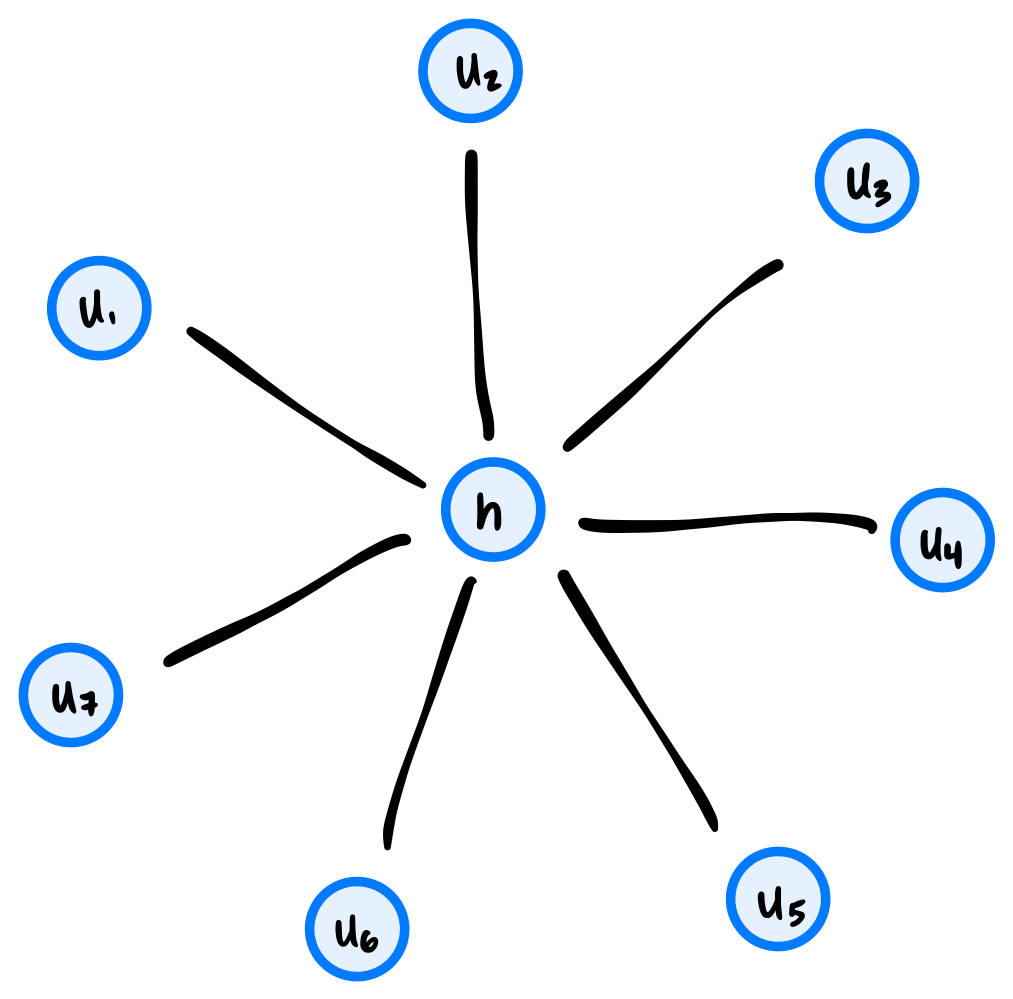
\includegraphics[width=.5\textwidth]{./g5.png}

    What is the \textbf{worst case} time complexity of an optimal algorithm
    which takes as input an arbitrary graph $G = (V, E)$ and determines if it
    is a ``hub and spoke'' graph? You may assume that the graph is represented as
    an adjacency list and that the total number of edges in the graph can be retrieved
    in constant time.

    \begin{choices}
        \correctchoice $\Theta(1)$
        \choice $\Theta(V)$
        \choice $\Theta(V + E)$
        \choice $\Theta(V^2)$
        \choice $\Theta(E^2)$
    \end{choices}

    \begin{soln}
        $\Theta(1)$

        Here's the algorithm. First, check that the number of edges is $|V| - 1$. If not, it's not a ``hub and spoke'' graph.
        This takes constant time, by the assumption that the total number of edges can be retrieved in constant time.

        Next, take an arbitrary node and compute its degree (in $\Theta(1)$ time), since
        the graph is represented as an adjacency list). If the degree is $n - 1$, then the graph is a
        ``hub and spoke'' graph, and this is the hub.

        If the degree is not $n - 1$, but instead 1, this node might be a spoke. Check the degree of its
        neighbor as described above to see if its a hub.

        If you see a degree that's neither 1 nor $n - 1$, then the graph is not a ``hub and spoke'' graph.
    \end{soln}

\end{prob}
